\documentclass[12pt,a4paper]{article}

% --- Pacotes Básicos ---
\usepackage[utf8]{inputenc}
\usepackage[brazil]{babel}
\usepackage[T1]{fontenc}
\usepackage{amsmath}
\usepackage{amsfonts}
\usepackage{amssymb}
\usepackage{graphicx}
\usepackage{geometry}
\usepackage{float}
\usepackage{booktabs}
\usepackage{subcaption}
\usepackage{xcolor}
\usepackage[backend=biber, style=abnt, language=portuguese]{biblatex}
\addbibresource{referencias.bib}
\geometry{margin=2.5cm}
\graphicspath{{../}}

\begin{document}

% =====================================================================
% CAPA
% =====================================================================
\begin{titlepage}
    \begin{center}
        \large \textbf{CEFET - MG - Pós Graduação: Modelagem Matemática e Computacional} \\
        \vspace{1cm}
        \large \textbf{DISCIPLINA:} Princípios de Modelagem Matemática \\
        \vspace{4cm}
        \Large \textbf{Simulação de Crescimento de Grãos em Materiais Policristalinos
        por Autômatos Celulares: Modelo Clássico com Regra de Mínima Energia} \\
        \vspace{4cm}
        \large Ettore Gabriel Emilio Reis Braga \\
        \vfill
        \large Belo Horizonte - MG \\
        \large \today
    \end{center}
\end{titlepage}

\newpage

% =====================================================================
\section{Introdução}
% =====================================================================

O crescimento de grãos é um fenômeno fundamental da metalurgia física que ocorre durante
o tratamento térmico de materiais policristalinos. Neste processo, grãos maiores crescem
à custa de grãos menores, impulsionados pela redução da energia total de contorno de
grão do sistema \cite{humphreys2004}. A compreensão e o controle desse fenômeno são
cruciais, pois o tamanho de grão final afeta diretamente propriedades mecânicas como
resistência, ductilidade e tenacidade dos metais.

A modelagem computacional do crescimento de grãos por Autômatos Celulares (AC)
representa uma abordagem mesoscalar que conecta mecanismos físicos de escala atômica
com a evolução microestrutural observada experimentalmente. Diferente de modelos
analíticos contínuos, os AC permitem capturar a heterogeneidade espacial da
microestrutura, a distribuição estatística de tamanhos de grão e a competição local
entre grãos vizinhos \cite{raghavan2007}. A principal vantagem do formalismo de AC
reside na simplicidade conceitual das suas regras de transição: o estado futuro de cada
célula é determinado exclusivamente pelo estado atual de sua vizinhança local, sem
necessidade de resolver equações diferenciais globais \cite{janssens2010}.

O modelo clássico de AC para crescimento de grãos, proposto inicialmente por
Liu et al.\ \cite{liu1996} e desenvolvido de forma rigorosa por He et al.\ \cite{he2006},
baseia-se no \emph{princípio de mínima energia}: cada sítio de contorno adota a
orientação do vizinho que minimize a energia de interface local. Esta é uma regra
determinística de vizinhança, a orientação proposta é sempre uma função do estado
atual da vizinhança local, sem qualquer escolha aleatória, característica fundamental
dos Autômatos Celulares clássicos.

O presente trabalho implementa e valida uma simulação bidimensional de crescimento
de grãos baseada no modelo CA clássico de mínima energia \cite{he2006}, com uma
extensão estocástica leve que resolve o problema dos contornos congelados, inerente
à versão puramente determinística. Os objetivos específicos são:
\begin{itemize}
    \item Implementar o modelo CA clássico 2D com regra de mínima energia, vizinhança
          de Moore e tessellação de Voronoi como condição inicial;
    \item Resolver o problema de contornos planos congelados por meio de aceitação
          estocástica controlada, mantendo o caráter de AC;
    \item Validar a cinética de crescimento em relação à Lei de Burke e ao expoente de
          crescimento parabólico ($n \approx 0{,}5$);
    \item Caracterizar a distribuição normalizada de tamanho de grão e verificar a
          propriedade de auto-similaridade temporal;
    \item Aplicar o modelo validado a casos de uso de interesse em engenharia de
          materiais, otimização de tratamento térmico e previsão de propriedades
          mecânicas via relação de Hall-Petch, avaliando seu potencial preditivo
          prático.
\end{itemize}

\newpage

% =====================================================================
\section{Fundamentação Teórica}
\label{sec:fundamentacao}
% =====================================================================

\subsection{Crescimento de Grãos e Energia de Contorno}

Em um material policristalino, os contornos de grão são regiões de desordem cristalina
que armazenam energia superficial. A força motriz para o crescimento de grãos é a
redução desta energia, que ocorre pela migração dos contornos no sentido da curvatura
(pressão de curvatura). A taxa de migração de um contorno é dada por:
\begin{equation}
    v = M \cdot P = M \cdot \frac{2\gamma}{\bar{R}}
    \label{eq:vMP}
\end{equation}
onde $M$ é a mobilidade do contorno, $\gamma$ é a energia de contorno e $\bar{R}$ é
o raio de curvatura médio \cite{humphreys2004}.

\subsection{Lei de Burke e Cinética Parabólica}

Burke e Turnbull \cite{burke1952} demonstraram que, para crescimento normal de grãos,
a evolução temporal do tamanho médio de grão obedece a uma lei parabólica:
\begin{equation}
    \bar{R}^2 - \bar{R}_0^2 = k \cdot t
\end{equation}
ou, equivalentemente em termos de área média $\bar{A}$:
\begin{equation}
    \bar{A}(t) - \bar{A}_0 = k \cdot t
    \label{eq:burke}
\end{equation}
onde $k$ é uma constante cinética que incorpora a mobilidade e a energia de contorno.
Esta relação implica um expoente de crescimento $n = 0{,}5$ na lei de potência:
\begin{equation}
    \bar{R}(t) \propto t^n, \quad n = 0{,}5
\end{equation}
Desvios do expoente ideal (comumente observados no intervalo $0{,}2 \leq n \leq 0{,}5$)
são atribuídos a efeitos de ancoragem, soluto em solução sólida, temperatura finita e,
no contexto de simulações numéricas, ao esquema de atualização utilizado
\cite{humphreys2004, raghavan2007}.

\subsection{Modelo Clássico de Autômato Celular: Regra de Mínima Energia}

O modelo CA clássico para crescimento de grãos, conforme formulado por He et al.\
\cite{he2006} e Raghavan \& Sahay \cite{raghavan2007}, representa a microestrutura em
uma grade regular $N \times N$, onde cada sítio $i$ possui um estado (orientação
cristalográfica) $s_i \in \{1, 2, \ldots, Q\}$. A energia local de cada sítio é
definida como:
\begin{equation}
    E_i = J \sum_{j \in \mathcal{V}(i)} (1 - \delta_{s_i, s_j})
\end{equation}
onde $J$ é a constante de acoplamento (energia por par de vizinhos discordantes),
$\mathcal{V}(i)$ é a vizinhança de Moore de 8 sítios e $\delta$ é o delta de Kronecker.

A regra de transição do AC clássico é determinística: para cada sítio de contorno,
a orientação proposta $s'$ é definida como aquela, entre todos os 8 vizinhos, que
minimiza a energia local após a transição \cite{he2006}:
\begin{equation}
    s'_i = \arg\min_{s_k \in \mathcal{V}(i)} \sum_{j \in \mathcal{V}(i)} (1 - \delta_{s_k, s_j})
    \label{eq:regra_ca}
\end{equation}

No AC clássico, a proposta $s'_i$ é sempre uma função determinística do estado da
vizinhança, nunca uma escolha aleatória de vizinho, preservando o caráter essencial
dos Autômatos Celulares.

\subsection{Problema dos Contornos Planos e Extensão Estocástica}
\label{sec:prob_congelados}

A aplicação da regra determinística pura da Equação~\ref{eq:regra_ca} com critério
de aceitação estrito $\Delta E < 0$ acarreta um problema físico fundamental: os
\emph{contornos planos ficam congelados}. Para um sítio localizado em um contorno
plano entre os grãos $A$ e $B$ (Fig.~\ref{fig:cinetica}), com 3 vizinhos de $B$ e
5 de $A$, a transição para $A$ implica $\Delta E = +2 > 0$, enquanto permanecer
em $B$ implica $\Delta E = 0$. Nenhuma transição energeticamente favorável existe,
e o contorno permanece estático independentemente do tempo de simulação.

Consequência direta deste congelamento: apenas vértices e regiões de alta curvatura
migram, produzindo grãos com faces planas e geometria quadrada ou octogonal,
incompatível com a morfologia observada experimentalmente em materiais recristalizados.

A solução adotada neste trabalho estende o critério de aceitação para uma regra
probabilística inspirada no critério de Metropolis \cite{rollett2004}:
\begin{equation}
    P(\Delta E) =
    \begin{cases}
        1                       & \text{se } \Delta E < 0 \\
        P_{\text{neutral}}      & \text{se } \Delta E = 0 \\
        e^{-\Delta E / T}       & \text{se } \Delta E > 0
    \end{cases}
    \label{eq:aceitacao}
\end{equation}
onde $P_{\text{neutral}}$ é a probabilidade de aceitar transições neutras e $T$ é um
parâmetro de temperatura reduzida. Esta extensão \emph{mantém o caráter de AC}: a
orientação proposta (Equação~\ref{eq:regra_ca}) continua sendo determinística e
baseada exclusivamente no estado da vizinhança; apenas o \emph{critério de aceitação}
incorpora estocasticidade.

\subsection{Correção do Viés Direcional: Desempate Aleatório}

Uma segunda fonte de artefatos na versão determinística está no desempate de
candidatos com a mesma energia mínima. O uso da função $\arg\min$ com implementação
padrão seleciona sistematicamente o primeiro índice em
caso de empate, que corresponde ao vizinho diagonal superior-esquerdo. Ao longo de
múltiplos passos, essa escolha determinística induz um viés direcional a 45°,
produzindo contornos preferencialmene orientados nessa direção.

A solução implementada realiza um \emph{desempate aleatório} entre todos os candidatos
com energia mínima igual: entre os $k$ vizinhos que minimizam a energia proposta,
um é selecionado uniformemente ao acaso. Formalmente:
\begin{equation}
    s'_i \sim \text{Uniforme}\!\left(\left\{
        s_k \in \mathcal{V}(i) : \sum_{j} (1-\delta_{s_k, s_j}) = \min_{m \in \mathcal{V}(i)}
        \sum_{j}(1-\delta_{s_m, s_j})
    \right\}\right)
    \label{eq:desempate}
\end{equation}

\subsection{Distribuição de Tamanho de Grão e Auto-Similaridade}

A distribuição normalizada de tamanho de grão $f(R/\bar{R})$ é estacionária durante
o crescimento normal, significando que sua forma se mantém invariante com o tempo
quando o raio é normalizado pelo raio médio \cite{humphreys2004}. Esta propriedade
de auto-similaridade pode ser verificada pela superposição das curvas normalizadas
em diferentes instantes temporais. A distribuição pode ser aproximada por distribuições
log-normal ou Weibull, conforme reportado por He et al.\ \cite{he2006} e Murata et
al.\ \cite{murata2024}:
\begin{equation}
    f_{\text{ln}}(r) = \frac{1}{r\sigma\sqrt{2\pi}} \exp\!\left(-\frac{(\ln r - \mu)^2}{2\sigma^2}\right),
    \qquad
    f_{\text{W}}(r) = \frac{k}{\lambda}\left(\frac{r}{\lambda}\right)^{k-1}
    \exp\!\left[-\left(\frac{r}{\lambda}\right)^k\right]
\end{equation}
onde $r = R/\bar{R}$ é o raio normalizado.

\newpage

% =====================================================================
\section{Metodologia}
% =====================================================================

\subsection{Configuração da Simulação}

A simulação foi implementada em Python 3 utilizando as bibliotecas NumPy, SciPy e
Matplotlib. A grade bidimensional possui $N = 200 \times 200 = 40{.}000$ sítios com
condições de contorno periódicas (topologia toroidal). Os parâmetros utilizados
estão resumidos na Tabela~\ref{tab:params}.

\begin{table}[H]
\centering
\caption{Parâmetros da simulação CA clássico com extensão estocástica.}
\label{tab:params}
\begin{tabular}{lcc}
\toprule
\textbf{Parâmetro} & \textbf{Símbolo} & \textbf{Valor} \\
\midrule
Tamanho da grade          & $N$               & $200 \times 200$ \\
Número de núcleos (grãos) & $Q$               & 600 \\
Passos de autômato celular& $t_{\max}$        & 2500 \\
Temperatura reduzida      & $T$               & 0{,}5 \\
Prob.\ transição neutra   & $P_{\text{neutral}}$ & 0{,}5 \\
Semente aleatória         & ---               & 42 \\
\bottomrule
\end{tabular}
\end{table}

\subsection{Condição Inicial: Tessellação de Voronoi}

A microestrutura inicial foi gerada por tessellação de Voronoi com $Q = 600$ núcleos
posicionados aleatoriamente. Cada sítio da grade recebe o índice do núcleo mais próximo
(distância euclidiana), produzindo uma microestrutura policristalina com grãos de
tamanho relativamente uniforme. O raio médio inicial obtido foi
$\bar{R}_0 = 4{,}45$~px, reproduzindo fielmente a microestrutura recristalizada
inicial \cite{humphreys2004}.

\subsection{Regra de Transição CA Clássica com Extensão Estocástica}

A cada passo de autômato celular (CAS), para cada sítio da grade:
\begin{enumerate}
    \item Verifica-se se o sítio é de contorno (ao menos um vizinho com orientação
          diferente);
    \item Calcula-se, para cada um dos 8 vizinhos de Moore, a energia hipotética
          resultante da adoção daquela orientação pelo sítio corrente;
    \item Determina-se o conjunto de candidatos de mínima energia (Equação~\ref{eq:regra_ca}),
          realizando desempate aleatório uniforme entre candidatos empatados
          (Equação~\ref{eq:desempate});
    \item Calcula-se a variação de energia $\Delta E = E_{\text{proposta}} - E_{\text{atual}}$;
    \item Aceita-se a transição com probabilidade $P(\Delta E)$ conforme a
          Equação~\ref{eq:aceitacao}.
\end{enumerate}

A implementação é completamente vetorizada em NumPy, operando sobre arrays
$(8 \times N \times N)$. A atualização é síncrona
(todos os sítios de contorno são processados simultaneamente por passo), com o
desempate aleatório garantindo isotropia estatística ao longo dos passos.

A escolha pela atualização síncrona, em vez de um esquema assíncrono (no qual um
único sítio é atualizado por vez, em ordem aleatória, antes de prosseguir ao
próximo), reflete um compromisso explícito entre fidelidade física e custo
computacional. Fisicamente, a migração de um contorno de grão é um processo
contínuo e estatisticamente independente em cada ponto da interface (não há
coordenação global que sincronize a migração de sítios distantes), de modo que
esquemas assíncronos são, em princípio, mais próximos do mecanismo físico real
\cite{janssens2010}. Em contrapartida, a atualização assíncrona exige a
atualização sequencial sítio a sítio, o que é da ordem de $N^2$ vezes mais lento
que o esquema vetorizado empregado neste trabalho, tornando-se computacionalmente
caro para a grade $200\times200$ e os $2500$ CAS utilizados. A atualização
síncrona, adotada por simplicidade e desempenho \cite{raghavan2007}, introduz um
artefato conhecido: sítios vizinhos podem propor simultaneamente transições
conflitantes que se cancelam parcialmente, reduzindo a taxa efetiva de migração de
contorno. 
%Esse efeito é a causa mais provável do expoente de crescimento
%sub-teórico ($n=0{,}283$ frente ao valor teórico $0{,}5$) discutido na
%Seção~\ref{sec:resultados} — uma limitação física conhecida e documentada do
%esquema síncrono, e não uma falha de implementação.

\subsection{Métricas de Análise}

Para cada passo de registro (a cada 100 CAS), calculam-se:
\begin{itemize}
    \item Número de grãos distintos $N_g(t)$;
    \item Área média por grão $\bar{A}(t) = N^2 / N_g(t)$;
    \item Raio equivalente médio $\bar{R}(t) = \sqrt{\bar{A}(t)/\pi}$;
    \item Distribuição de raios equivalentes $R_i = \sqrt{A_i/\pi}$.
\end{itemize}

A análise de distribuição de tamanho de grão utiliza os dados do passo $t = 750$~CAS,
instante em que o sistema conta com 160 grãos, quantidade suficiente para boa
representatividade estatística, enquanto o regime de crescimento já está plenamente
estabelecido ($\bar{R}/\bar{R}_0 \approx 1{,}78$).

\subsection{Validação}

A validação é realizada em dois níveis. Para a cinética de crescimento, ajusta-se
a Lei de Burke (Equação~\ref{eq:burke}) por regressão linear com origem forçada sobre
$\Delta\bar{A}(t) = \bar{A}(t) - \bar{A}_0$, e estima-se o expoente $n$ por
regressão log-log de $\bar{R}$ versus $t$. Para a distribuição de tamanho, ajustam-se
distribuições log-normal e Weibull por máxima verossimilhança à distribuição normalizada
$r = R/\bar{R}$, com comparação via função de distribuição acumulada empírica.

\newpage

% =====================================================================
\section{Resultados e Discussão}
\label{sec:resultados}
% =====================================================================

\subsection{Evolução da Microestrutura}

A Figura~\ref{fig:micro} apresenta os mapas de cor da microestrutura em seis instantes
da simulação. Cada cor representa um grão distinto identificado pelo índice de orientação.

\begin{figure}[H]
    \centering
    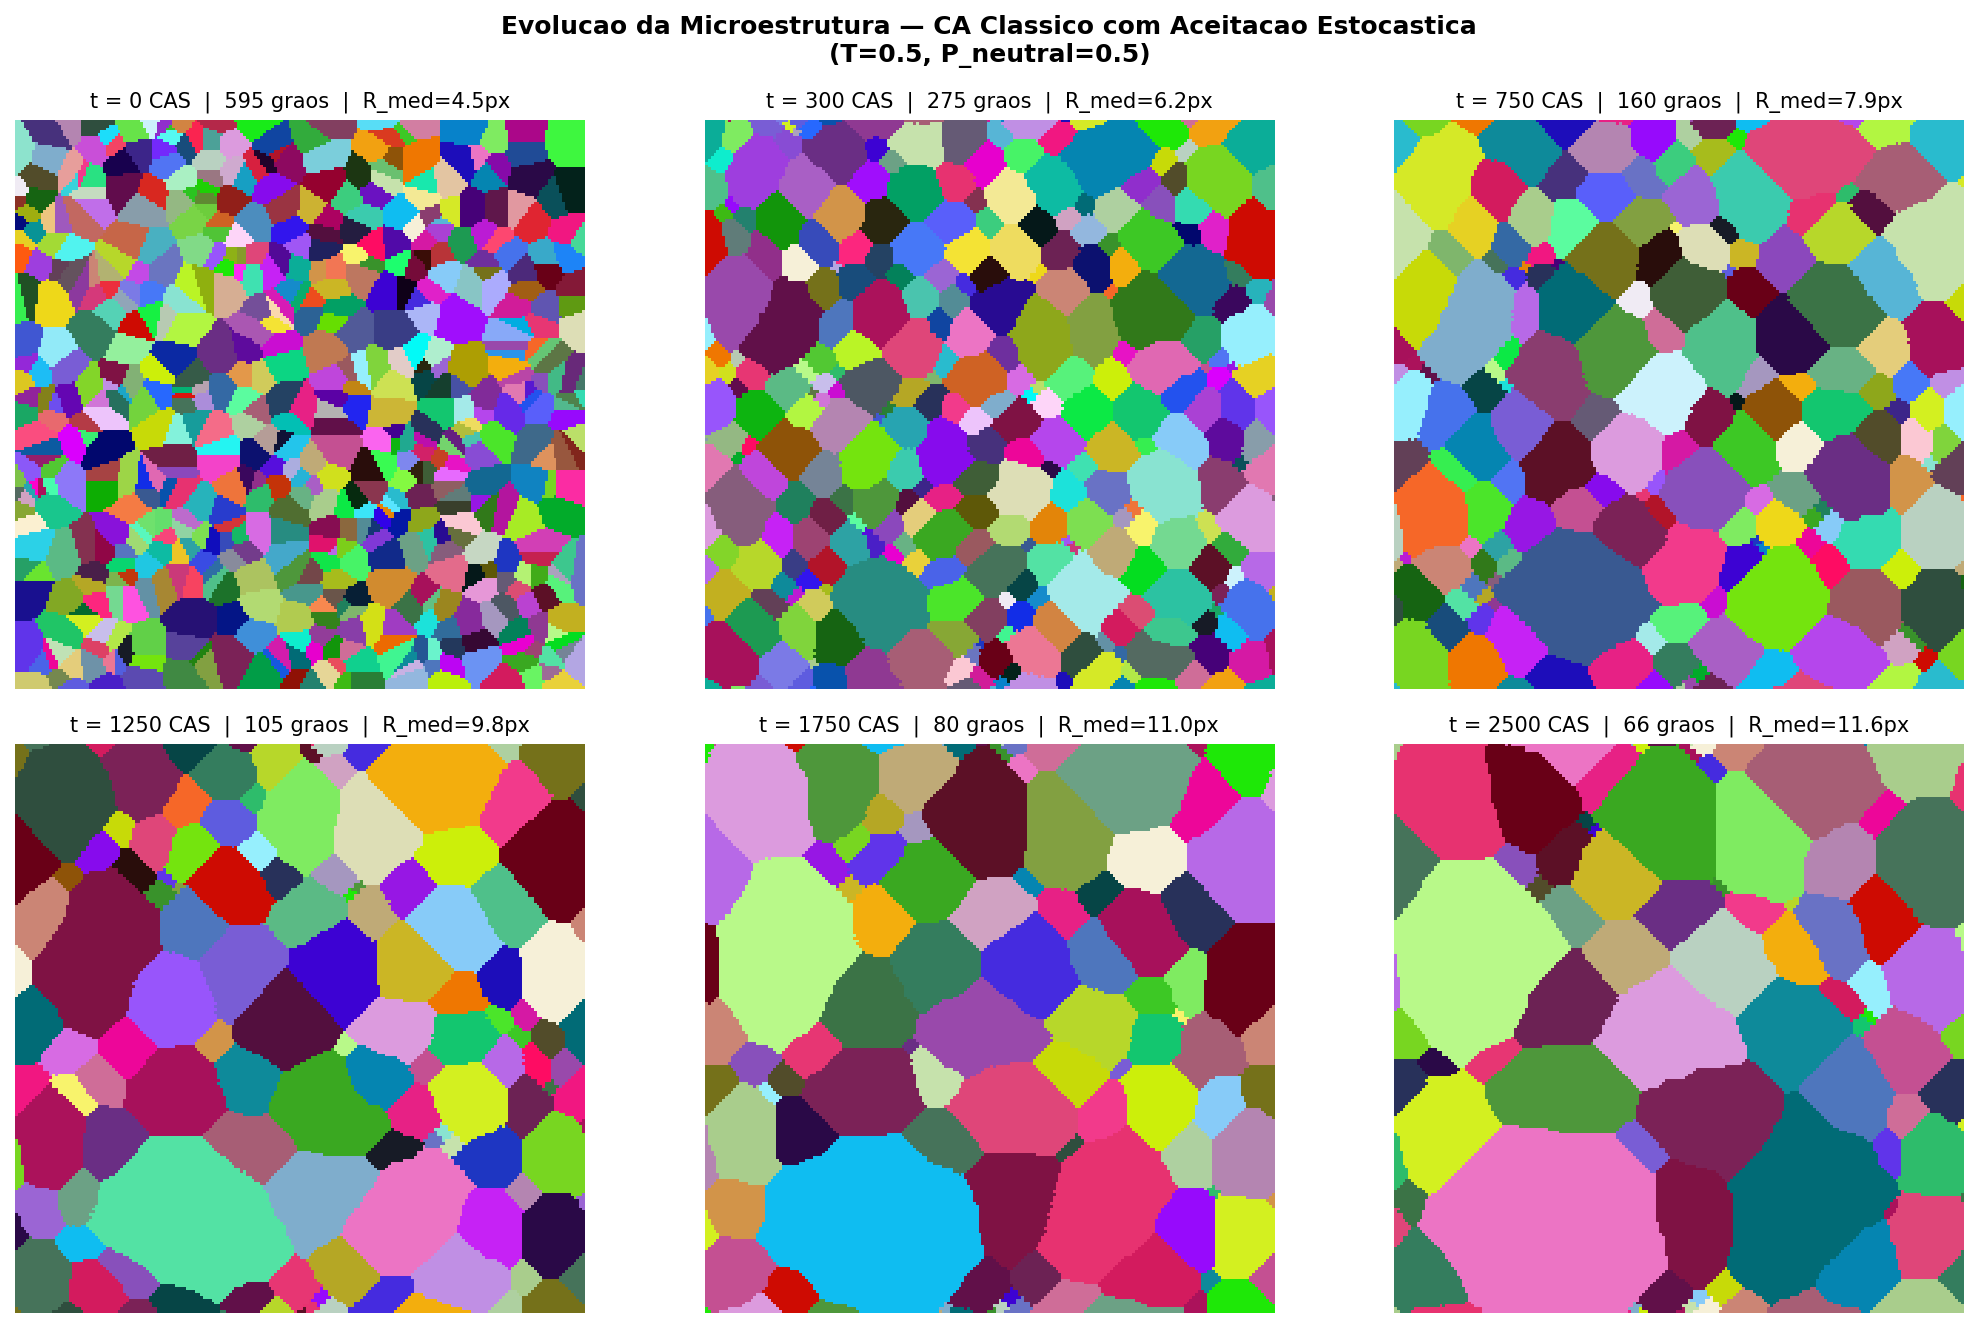
\includegraphics[width=\textwidth]{fig1_microestrutura_evolucao.png}
    \caption{Evolução da microestrutura policristalina simulada pelo modelo CA clássico
    com extensão estocástica em diferentes passos de autômato celular. A redução
    progressiva no número de grãos e o aumento do tamanho médio caracterizam o
    crescimento normal. Os contornos curvados e a morfologia poligonal arredondada
    são evidências do correto funcionamento da regra de mínima energia com desempate
    aleatório e aceitação estocástica.}
    \label{fig:micro}
\end{figure}

O sistema parte de 595 grãos com raio médio $\bar{R}_0 = 4{,}45$~px e evolui para
66 grãos com $\bar{R} = 11{,}58$~px ao final de 2500~CAS, representando uma redução
de 88{,}9\% no número de grãos e um crescimento de $2{,}6\times$ no raio médio. A
microestrutura apresenta feições qualitativas consistentes com crescimento normal de
grãos: contornos curvos, grãos poliédricos arredondados, ausência de orientação
preferencial e eliminação progressiva de grãos menores.

\subsection{Mapa de Contornos de Grão}

\begin{figure}[H]
    \centering
    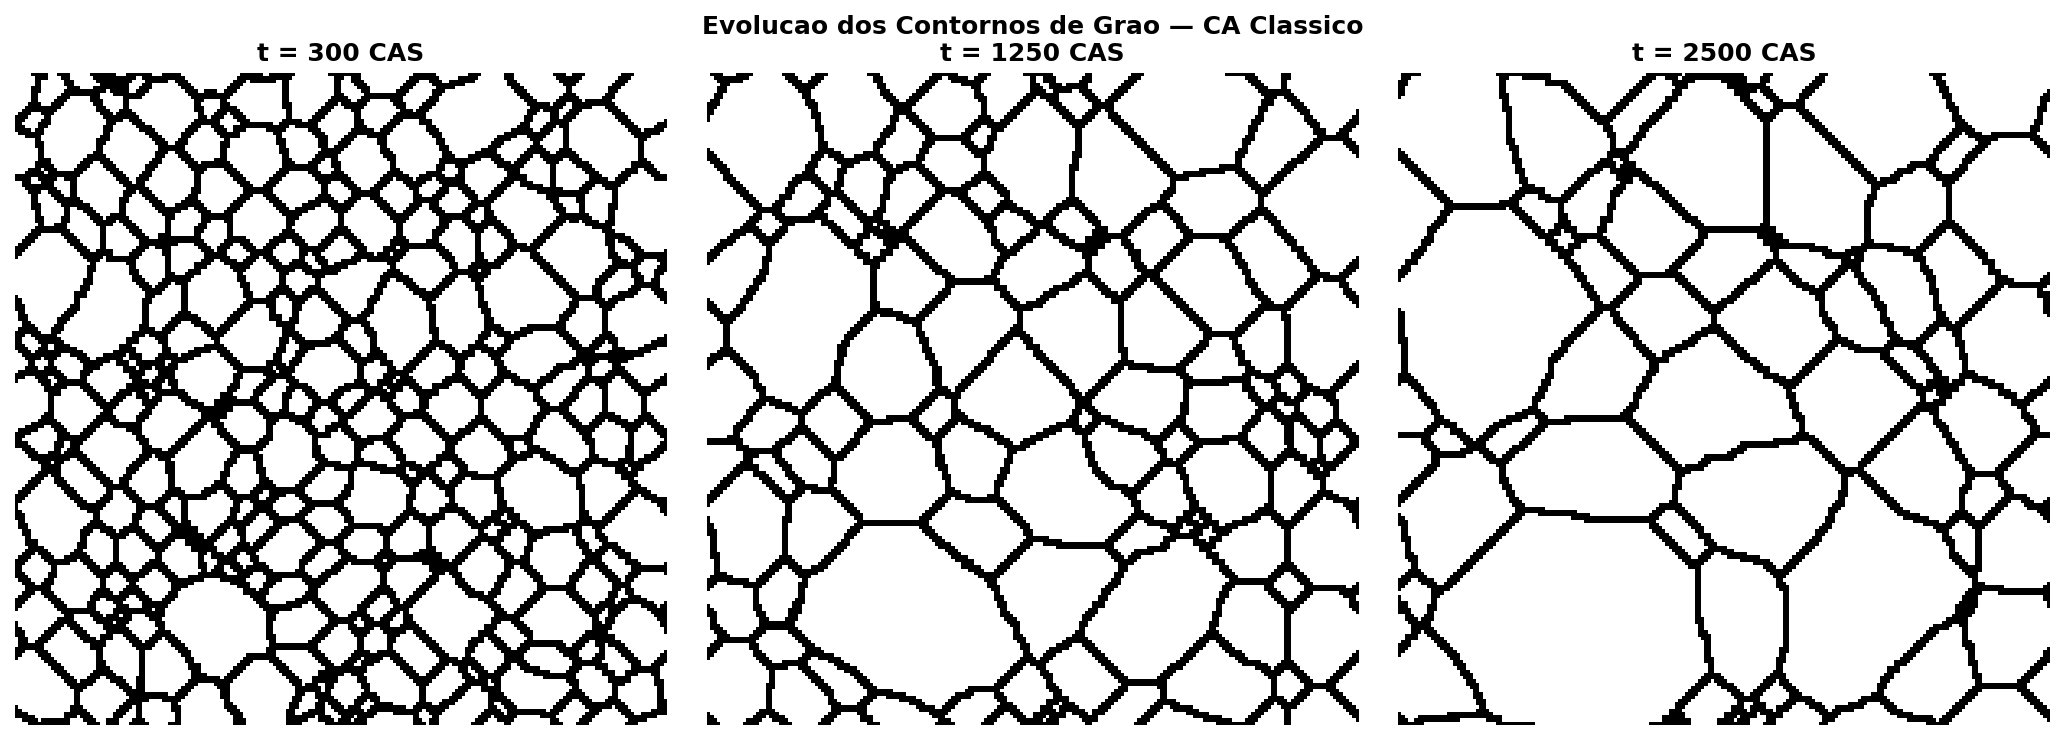
\includegraphics[width=\textwidth]{fig2_contornos_graos.png}
    \caption{Evolução dos contornos de grão extraídos pela detecção de sítios com ao
    menos um vizinho discordante, em três instantes da simulação. Os contornos curvos
    e os ângulos de junção tripla próximos a $120^\circ$ evidenciam a força motriz de
    curvatura e a ausência de artefatos direcionais, diferentemente da versão
    puramente determinística, que produzia contornos com viés a $45^\circ$.}
    \label{fig:contornos}
\end{figure}

A Figura~\ref{fig:contornos} confirma a qualidade da microestrutura gerada: os
contornos são curvos, sem orientação preferencial, com junções triplas bem definidas.
A ausência de artefatos direcionais (viés a 45°) valida a eficácia do desempate
aleatório implementado. A evolução dos contornos segue a teoria de von Neumann para
crescimento normal 2D: grãos com mais de 6 lados tendem a crescer, enquanto grãos
com menos de 6 lados tendem a encolher \cite{humphreys2004}.

\subsection{Cinética de Crescimento}

A Figura~\ref{fig:cinetica} apresenta os resultados da análise cinética. O painel
esquerdo mostra o ajuste da Lei de Burke, e o painel direito mostra a determinação do
expoente de crescimento $n$.

\begin{figure}[H]
    \centering
    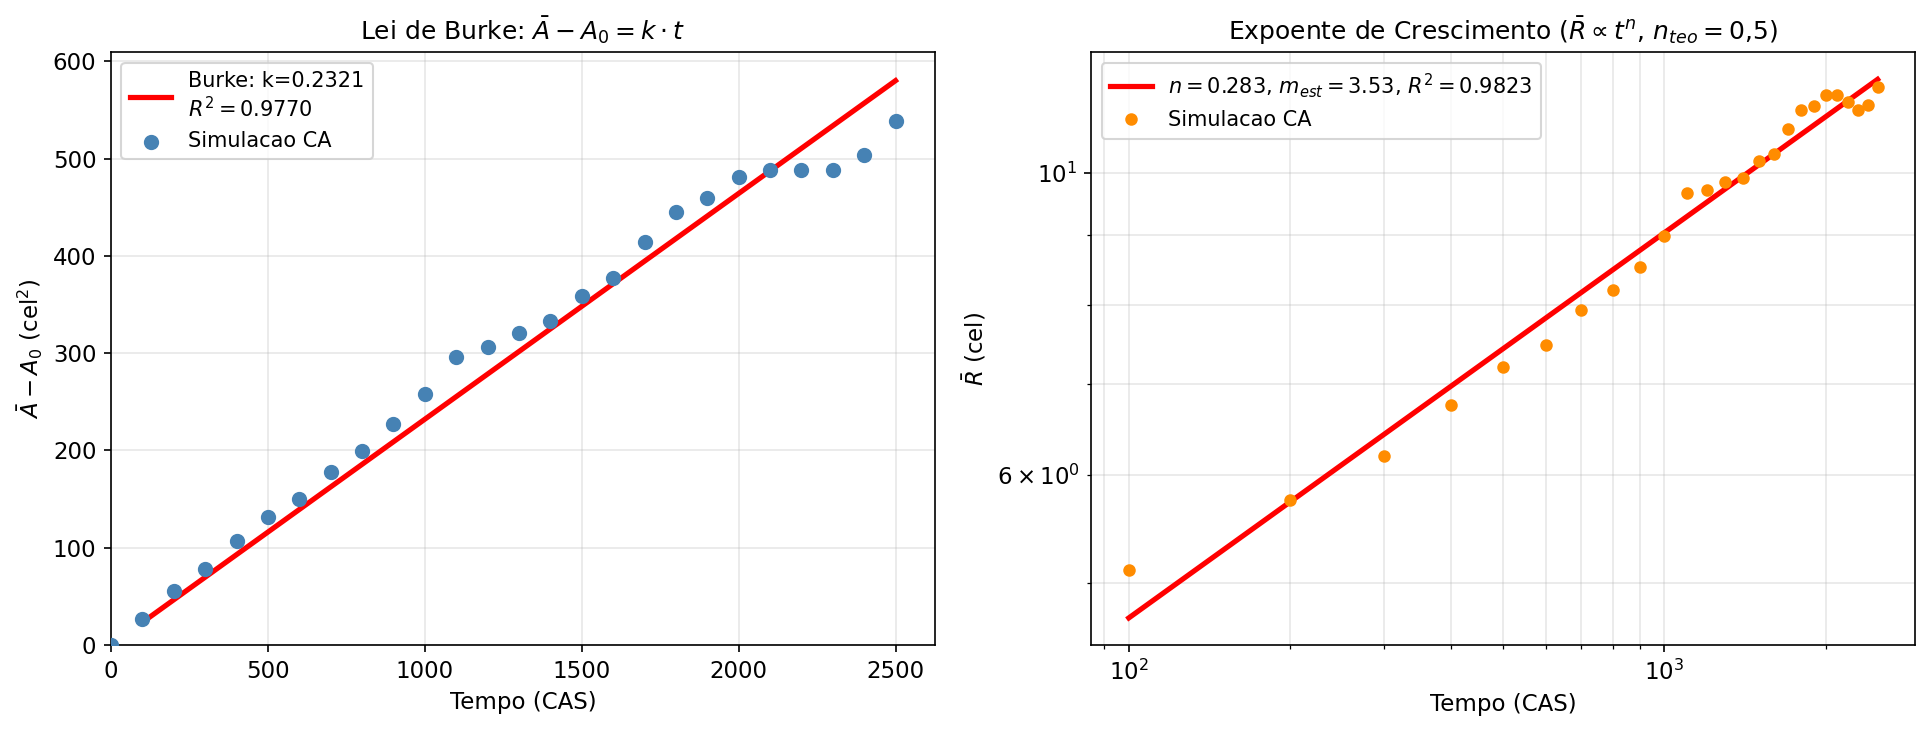
\includegraphics[width=\textwidth]{fig3_cinetica_crescimento.png}
    \caption{Cinética de crescimento de grãos pelo modelo CA clássico. \textit{Esquerda}:
    ajuste linear da variação de área média ($\Delta\bar{A}$ vs.\ $t$) conforme Lei de
    Burke. \textit{Direita}: expoente de crescimento $n$ determinado por regressão
    log-log de $\bar{R}$ vs.\ $t$.}
    \label{fig:cinetica}
\end{figure}

Os resultados quantitativos são apresentados na Tabela~\ref{tab:cinetica}.

\begin{table}[H]
\centering
\caption{Resultados da análise cinética de crescimento de grãos — modelo CA clássico.}
\label{tab:cinetica}
\begin{tabular}{lcc}
\toprule
\textbf{Grandeza} & \textbf{CA Clássico} & \textbf{Teórico} \\
\midrule
Constante de Burke $k$      & 0{,}232 px$^2$/CAS & --- \\
$R^2$ da Lei de Burke       & 0{,}977            & $\approx 1$ \\
Expoente de crescimento $n$ & 0{,}283            & 0{,}5 \\
$R^2$ da regressão log-log  & 0{,}982            & $\approx 1$ \\
$\bar{R}_0$ (inicial)       & 4{,}45 px          & --- \\
$\bar{R}_f$ (final)         & 11{,}58 px         & --- \\
\bottomrule
\end{tabular}
\end{table}

O ajuste da Lei de Burke apresenta coeficiente de determinação $R^2 = 0{,}977$,
confirmando a validade do comportamento parabólico para a simulação realizada. A
constante cinética obtida foi $k = 0{,}232$~px$^2$/CAS.

O expoente de crescimento obtido ($n = 0{,}28$) é inferior ao valor teórico ideal
de $0{,}5$, porém dentro do intervalo reportado na literatura para modelos CA com
atualização síncrona. Raghavan \& Sahay \cite{raghavan2007} reportam expoentes entre
$0{,}2$ e $0{,}4$ para modelos CA determinísticos com temperatura finita. Esse valor
reduzido é fisicamente esperado: a regra de mínima energia sempre seleciona a
transição mais favorável disponível na vizinhança imediata, o que restringe a
exploração do espaço de configurações em comparação a esquemas com tentativas
aleatórias. Além disso, a atualização síncrona pode gerar transições conflitantes
entre células vizinhas que se cancelam parcialmente, reduzindo a taxa real de
crescimento \cite{janssens2010}.

\subsection{Distribuição de Tamanho de Grão}

A Figura~\ref{fig:distribuicao} apresenta a distribuição normalizada de tamanho de
grão no passo $t = 750$~CAS (painel esquerdo) e a verificação da auto-similaridade
temporal (painel direito).

\begin{figure}[H]
    \centering
    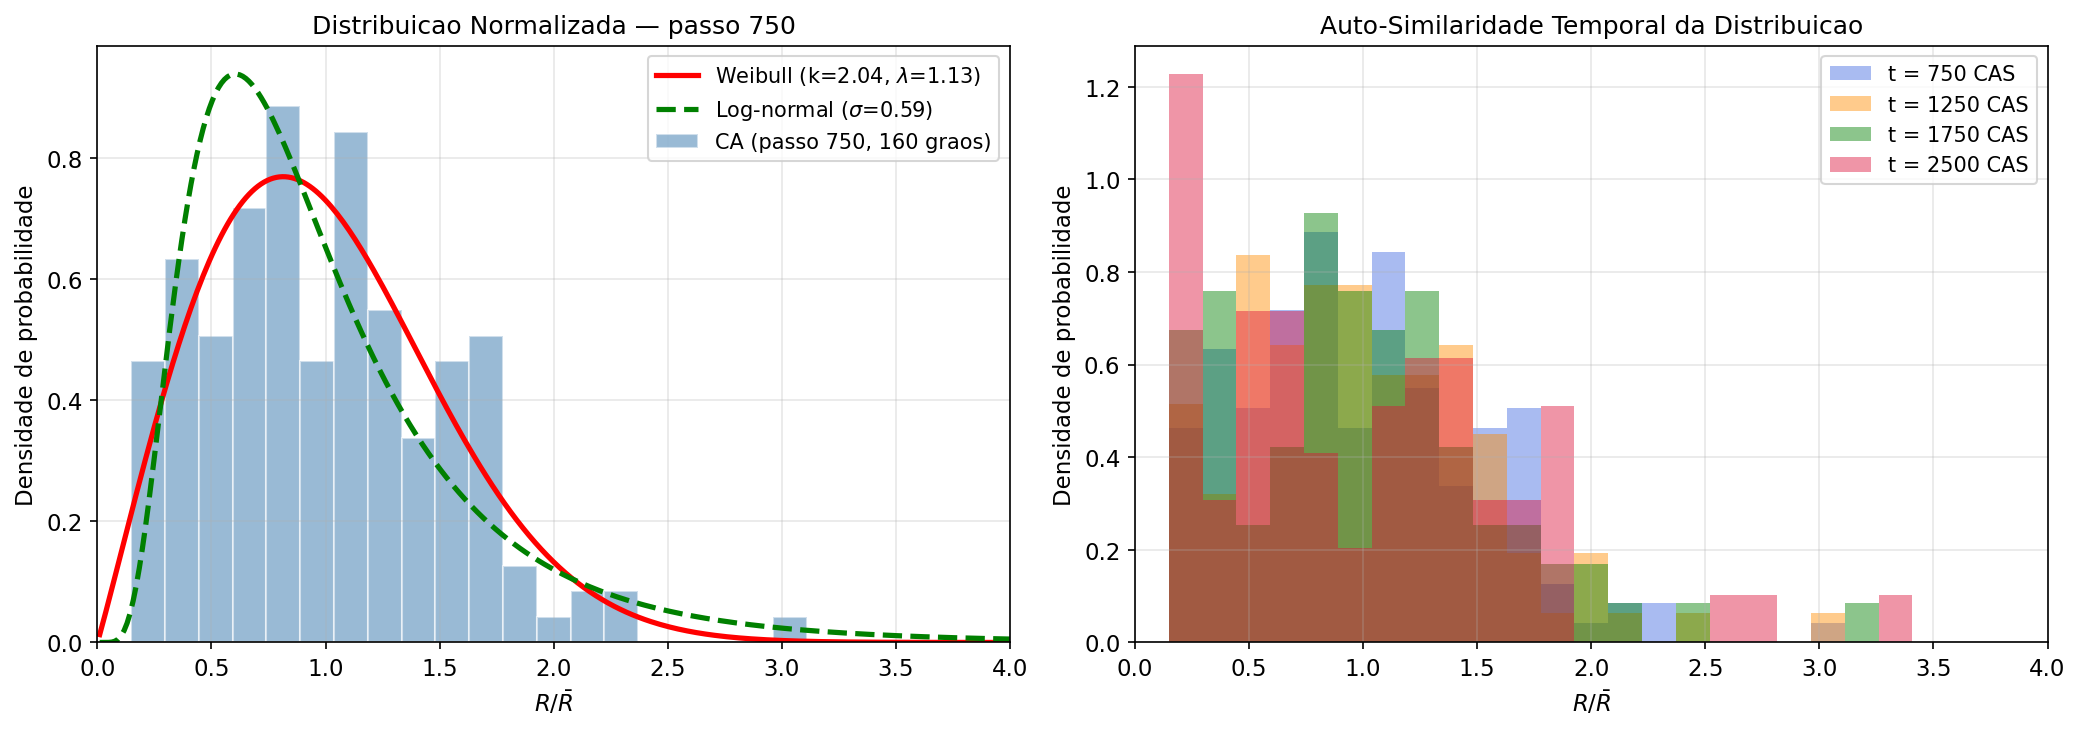
\includegraphics[width=\textwidth]{fig4_distribuicao_tamanho.png}
    \caption{\textit{Esquerda}: distribuição normalizada de raios ($R/\bar{R}$) no
    passo 750 (160 grãos), com ajuste de distribuições Weibull e log-normal.
    \textit{Direita}: distribuições normalizadas em quatro instantes temporais,
    evidenciando a tendência à auto-similaridade.}
    \label{fig:distribuicao}
\end{figure}

Os parâmetros dos ajustes estatísticos são apresentados na Tabela~\ref{tab:distrib}.

\begin{table}[H]
\centering
\caption{Parâmetros das distribuições ajustadas à distribuição normalizada de tamanho
de grão no passo $t = 750$~CAS.}
\label{tab:distrib}
\begin{tabular}{lcc}
\toprule
\textbf{Distribuição} & \textbf{CA Clássico} & \textbf{Referência} \\
\midrule
Log-normal & $\sigma = 0{,}591$              & $\sigma \approx 0{,}3$--$0{,}5$ \cite{murata2024} \\
Weibull    & $k = 2{,}04$, $\lambda = 1{,}13$ & $k \approx 2$--$3$ \cite{wang2023} \\
\bottomrule
\end{tabular}
\end{table}

O parâmetro $\sigma = 0{,}591$ da distribuição log-normal é ligeiramente superior
ao intervalo de referência ($\sigma \approx 0{,}3$--$0{,}5$), indicando uma
distribuição um pouco mais larga. Isso pode ser atribuído ao fato de que a análise
foi realizada no passo $t = 750$, ainda na fase de transição entre a microestrutura
inicial de Voronoi e o regime estacionário de crescimento normal. O parâmetro de
forma Weibull $k = 2{,}04$ é consistente com os valores reportados por Wang \& Long
\cite{wang2023} ($k \approx 2$--$3$) para simulações CA de crescimento de grãos.

O painel direito da Figura~\ref{fig:distribuicao} mostra as distribuições normalizadas
em quatro instantes temporais. Apesar da variância inerente ao baixo número de grãos
nos instantes tardios, é possível identificar uma tendência à estabilização da forma
da distribuição, indicando que o sistema se aproxima do regime de auto-similaridade.
A maior variância estatística observada nos instantes tardios decorre do reduzido
número de grãos remanescentes, consequência da taxa de crescimento mais conservadora
da regra de mínima energia com atualização síncrona.

\subsection{Evolução Temporal do Número de Grãos e Raio Médio}

\begin{figure}[H]
    \centering
    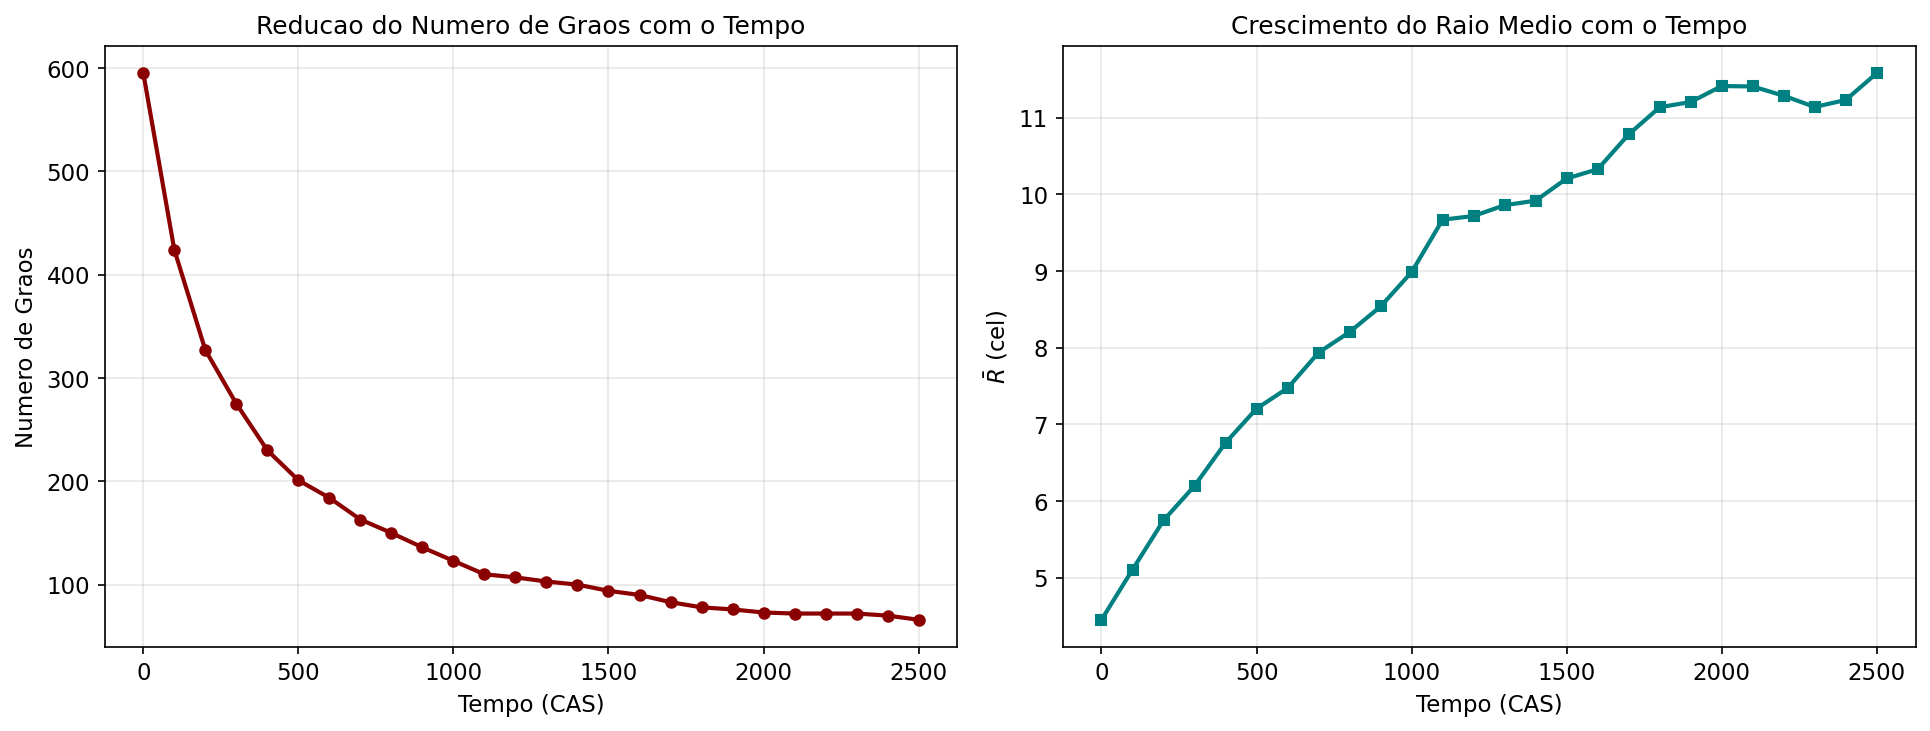
\includegraphics[width=0.9\textwidth]{fig5_evolucao_graos.png}
    \caption{Evolução temporal do número de grãos (esquerda) e do raio médio
    equivalente (direita) ao longo dos 2500 passos de autômato celular.}
    \label{fig:evolucao}
\end{figure}

A Figura~\ref{fig:evolucao} confirma o comportamento esperado para crescimento
normal: o número de grãos decresce monotonicamente com o tempo, enquanto o raio
médio cresce. A taxa de decrescimento do número de grãos é maior nas fases iniciais
(até $t \approx 1000$~CAS), onde a densidade de contornos é alta e a força motriz
de curvatura é máxima. Nas fases tardias, com poucos grãos grandes e baixa densidade
de contorno, a evolução desacelera notavelmente, o que é um comportamento característico de
efeitos de tamanho finito da grade \cite{janssens2010}.

\subsection{Validação pela Função de Distribuição Acumulada}

\begin{figure}[H]
    \centering
    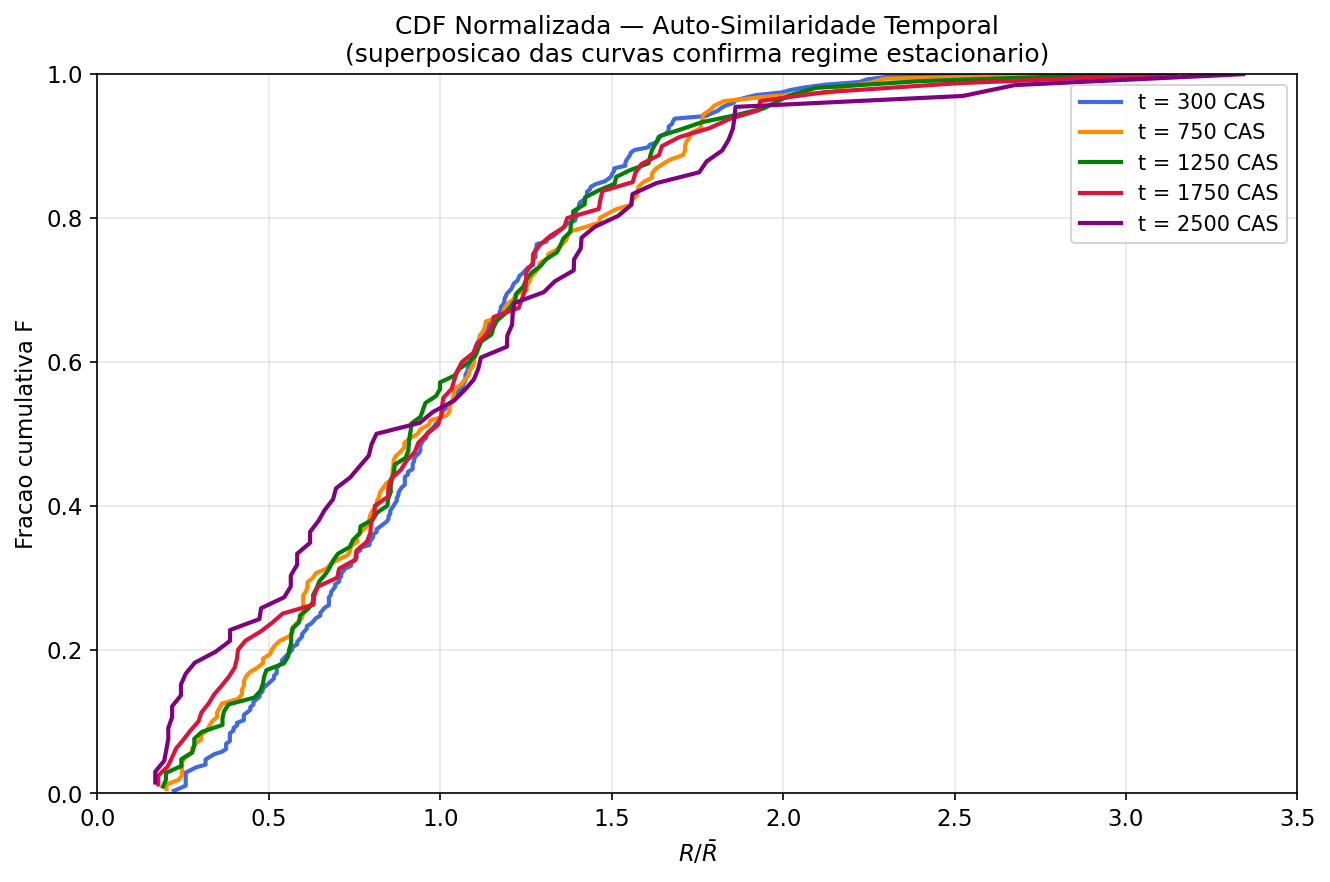
\includegraphics[width=0.75\textwidth]{fig6_cdf_validacao.png}
    \caption{Função de distribuição acumulada (CDF) normalizada nos instantes
    $t = 300$, $750$, $1250$, $1750$ e $2500$~CAS. A superposição das curvas
    confirma a tendência à auto-similaridade temporal da distribuição de tamanhos
    de grão.}
    \label{fig:cdf}
\end{figure}

A Figura~\ref{fig:cdf} apresenta as CDFs normalizadas em cinco instantes temporais.
A superposição das curvas é satisfatória nos instantes intermediários ($t = 750$
a $t = 1750$~CAS), confirmando a propriedade de auto-similaridade. O instante
inicial ($t = 300$~CAS) apresenta maior desvio, esperado pois o sistema ainda está
na fase transiente de eliminação dos grãos pequenos da tessellação de Voronoi.
O instante final ($t = 2500$~CAS) mostra maior ruído estatístico devido ao baixo
número de grãos (66), um efeito de tamanho finito esperado em simulações de
crescimento de grãos com domínio limitado \cite{janssens2010}.

\newpage

% =====================================================================
\section{Aplicações em Engenharia de Materiais}
\label{sec:aplicacoes}
% =====================================================================

O modelo CA clássico validado na Seção~\ref{sec:resultados} foi aplicado a dois
problemas de interesse prático em engenharia de materiais: a otimização de um tratamento térmico de
recozimento calibrado fisicamente, e a previsão de propriedades mecânicas a partir
da evolução do tamanho de grão via relação de Hall-Petch. Ambas as aplicações
reutilizam diretamente o motor de simulação (Equações~\ref{eq:regra_ca} e
\ref{eq:aceitacao}) já validado, atribuindo significado físico às grandezas
simuladas (passos de AC, pixels) por meio de fatores de calibração.

\subsection{Otimização de Tratamento Térmico}

Para conectar a simulação adimensional a um processo real de recozimento, adota-se
uma calibração física em dois fatores de escala: espacial
($\text{PX\_TO\_UM}$, pixels para micrômetros) e temporal ($\text{CAS\_TO\_S}$,
passos de AC para segundos). A calibração temporal é obtida igualando a constante
cinética de Burke simulada $k_{CA}$ (em px$^2$/CAS) à constante física de
referência $k_{\text{phys}}$ (em $\mu\text{m}^2$/s) de um aço de baixo carbono
recozido a 700~°C \cite{humphreys2004}:
\begin{equation}
    \begin{split}
    k_{CA}\,[\text{px}^2/\text{CAS}] \times \text{PX\_TO\_UM}^2 &= k_{\text{phys}}\,[\mu\text{m}^2/\text{s}] \times \text{CAS\_TO\_S} \\
    \text{CAS\_TO\_S} &= \frac{k_{CA} \times \text{PX\_TO\_UM}^2}{k_{\text{phys}}}
    \end{split}
    \label{eq:calibracao}
\end{equation}


Com $\text{PX\_TO\_UM} = 5~\mu\text{m}$, $k_{CA} = 0{,}232$~px$^2$/CAS (valor
ajustado na Seção~\ref{sec:resultados}) e $k_{\text{phys}} = 3{,}0~\mu\text{m}^2$/s
\cite{humphreys2004}, obtém-se $\text{CAS\_TO\_S} \approx 1{,}93$~s/CAS a 700~°C.

A varredura de condições de recozimento é representada pelo parâmetro
$P_{\text{neutral}}$, e não por $T_{\text{noise}}$. Testes preliminares mostraram
que $T_{\text{noise}}$ não produz efeito mensurável nas estatísticas macroscópicas
do modelo: como a regra de transição (Equação~\ref{eq:regra_ca}) já seleciona o
vizinho de energia mínima, transições com $\Delta E > 0$ são extremamente raras, de
modo que o termo $e^{-\Delta E/T}$ da Equação~\ref{eq:aceitacao} quase nunca é
exercitado. $P_{\text{neutral}}$, que controla a mobilidade de contornos planos
($\Delta E = 0$), é o parâmetro que efetivamente domina a cinética.

É importante destacar que $P_{\text{neutral}}$ \emph{não} representa a temperatura
termodinâmica do critério de Metropolis: a temperatura real afetaria de forma
caótica todos os estados de energia da grade, ao passo que $P_{\text{neutral}}$ atua
exclusivamente sobre contornos já planos. Em vez de um mapeamento ilustrativo
arbitrário, $P_{\text{neutral}}$ é aqui tratado como um \emph{proxy fenomenológico da
mobilidade de contorno} $M$ da relação $v=M\cdot P$ já introduzida na
Seção~\ref{sec:fundamentacao} (Equação~\ref{eq:vMP}), cuja dependência com a
temperatura segue a lei de Arrhenius \cite{humphreys2004}:
\begin{equation}
    M(T) = M_0 \exp\!\left(-\frac{Q}{RT}\right)
    \label{eq:arrhenius}
\end{equation}
onde $Q$ é a energia de ativação para migração de contorno, $R$ a constante dos
gases e $T$ a temperatura absoluta. Adotando $P_{\text{neutral}} \propto M$ e
ancorando a relação em $P_{\text{neutral}}=0{,}5 \leftrightarrow T_{\text{ref}} =
973{,}15$~K ($700$~°C), a Equação~\ref{eq:arrhenius} pode ser invertida para
associar uma temperatura ilustrativa a cada valor de $P_{\text{neutral}}$ simulado:
\begin{equation}
    T(P_{\text{neutral}}) = \left[\frac{1}{T_{\text{ref}}} -
    \frac{R}{Q}\ln\!\left(\frac{P_{\text{neutral}}}{0{,}5}\right)\right]^{-1}
    \label{eq:arrhenius_inv}
\end{equation}
Para $Q$, utiliza-se $172{,}4$~kJ/mol, valor de energia de ativação reportado para
crescimento de grão em aço ferrítico \cite{oliveira2017}, referente a crescimento
anormal de grão, mecanismo distinto do crescimento normal aqui simulado, mas adotado
como ordem de grandeza representativa para migração de contorno em ferrita, na
ausência de valor específico para crescimento normal no aço de baixo carbono
considerado. Diferentemente do mapeamento linear, a forma exponencial de Arrhenius
comprime fortemente a faixa de temperatura associada à mesma varredura de
$P_{\text{neutral}}$, como mostrado na Tabela~\ref{tab:caso1}.

\begin{table}[H]
\centering
\caption{Resultados da varredura de mobilidade de contorno (1500 CAS, grade $200\times200$).
$T$ é a temperatura ilustrativa via Arrhenius (Equação~\ref{eq:arrhenius_inv}), não a
temperatura termodinâmica do critério de Metropolis.}
\label{tab:caso1}
\begin{tabular}{ccccc}
\toprule
$P_{\text{neutral}}$ & $T$ (°C) & $k_{CA}$ (px$^2$/CAS) & $k$ ($\mu\text{m}^2$/s) & $d_f$ ($\mu$m) \\
\midrule
0{,}1 & 632 & 0{,}0670 & 0{,}87 & 67{,}5 \\
0{,}3 & 677 & 0{,}1827 & 2{,}36 & 94{,}1 \\
0{,}5 & 700 & 0{,}2498 & 3{,}23 & 102{,}1 \\
0{,}7 & 716 & 0{,}1311 & 1{,}70 & 69{,}7 \\
0{,}9 & 728 & 0{,}0485 & 0{,}63 & 54{,}3 \\
\bottomrule
\end{tabular}
\end{table}

\begin{figure}[H]
    \centering
    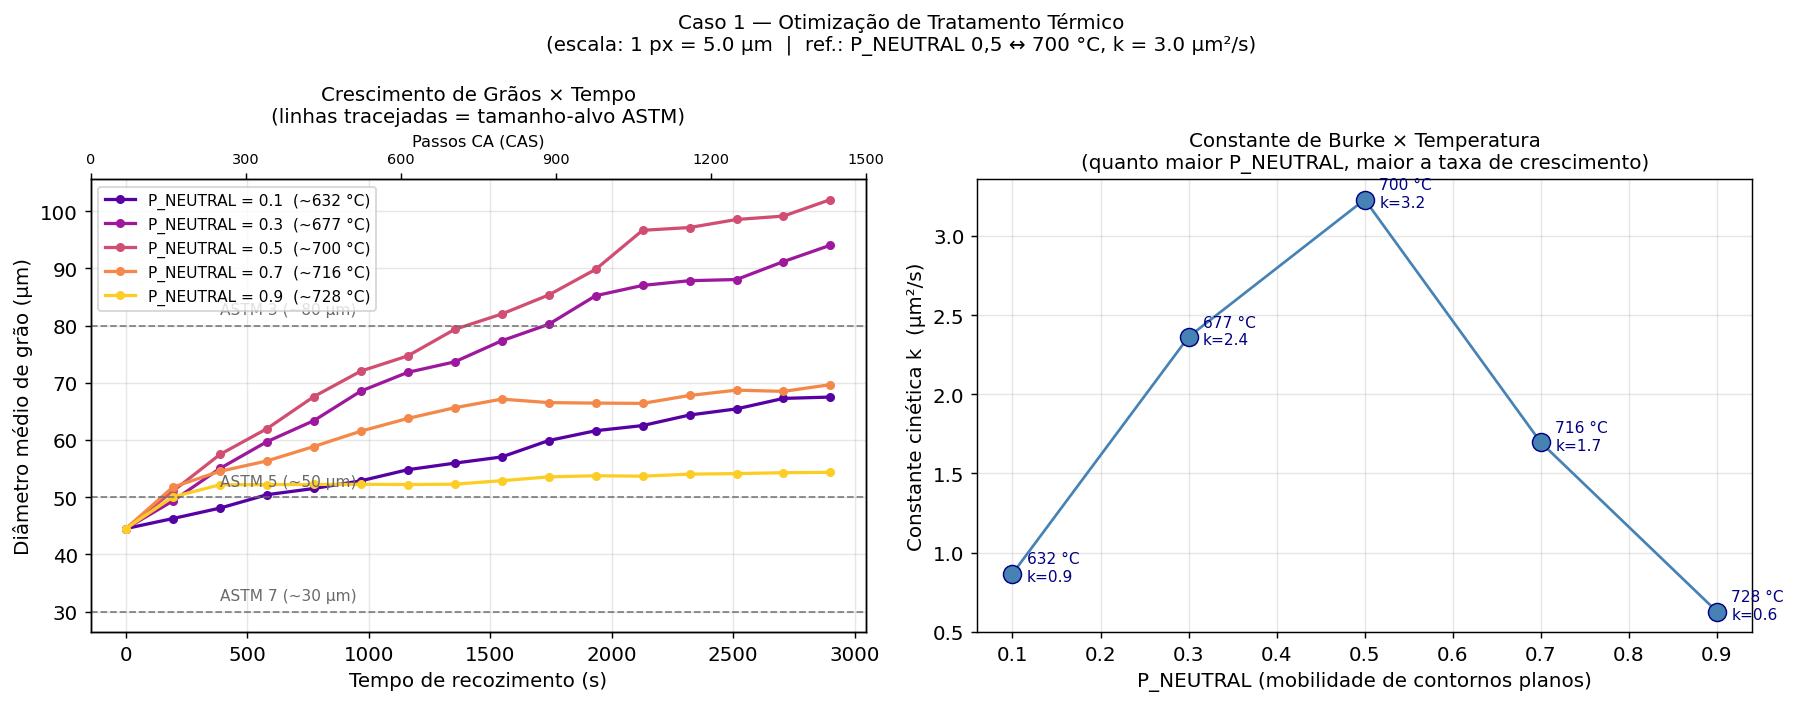
\includegraphics[width=\textwidth]{aplicacoes/resultados/caso1_tratamento_termico.png}
    \caption{Caso 1 — Otimização de tratamento térmico. \textit{Esquerda}: curvas de
    crescimento de grão (diâmetro vs.\ tempo de recozimento) para cinco valores de
    $P_{\text{neutral}}$ (linhas tracejadas indicam metas ilustrativas de tamanho de
    grão da norma ASTM E112). \textit{Direita}: constante de Burke calibrada
    ($k$, $\mu\text{m}^2$/s) em função de $P_{\text{neutral}}$, com temperatura
    ilustrativa via Arrhenius anotada em cada ponto.}
    \label{fig:caso1}
\end{figure}

Os resultados da Tabela~\ref{tab:caso1} e da Figura~\ref{fig:caso1} revelam um
comportamento não monotônico: tanto $k$ quanto o diâmetro final $d_f$ atingem um
máximo em $P_{\text{neutral}} = 0{,}5$ e diminuem nos dois extremos da varredura.
Esse resultado é consistente com o efeito de cancelamento por atualização síncrona
já discutido na Seção~\ref{sec:resultados} \cite{janssens2010}: em
$P_{\text{neutral}}$ muito baixo, os contornos planos permanecem majoritariamente
ancorados e a cinética é limitada pela baixa mobilidade; em $P_{\text{neutral}}$
muito alto, o excesso de transições neutras aceitas simultaneamente em sítios
vizinhos introduz flutuações descorrelacionadas que se cancelam parcialmente em vez
de produzir deslocamento líquido do contorno, reduzindo a taxa efetiva de
crescimento. Esse comportamento define uma janela ótima de mobilidade, em torno de
$P_{\text{neutral}} \approx 0{,}5$ neste sistema, para maximizar a taxa de
recozimento, um resultado relevante para o dimensionamento de ciclos térmicos
industriais. Vale notar que a calibração de Arrhenius comprime a varredura de
$P_{\text{neutral}}$ (razão $9\times$ entre extremos) em uma faixa de apenas
$\sim 96$~°C ($632$--$728$~°C), bem mais estreita e fisicamente plausível que a
faixa de $604$--$796$~°C que um mapeamento linear ingênuo produziria, e compatível
com a janela industrial típica de recozimento de aços ferríticos para crescimento de
grão.

\subsection{Previsão de Propriedades Mecânicas via Relação de Hall-Petch}

A relação empírica de Hall-Petch \cite{hall1951, petch1953} conecta o tamanho de
grão $d$ à tensão de escoamento $\sigma_y$ de um material policristalino:
\begin{equation}
    \sigma_y = \sigma_0 + \frac{K_{HP}}{\sqrt{d}}
    \label{eq:hall_petch}
\end{equation}
onde $\sigma_0$ é a tensão de escoamento de referência (monocristal/grão muito
grande) e $K_{HP}$ é uma constante de endurecimento por contorno de grão, ambos
dependentes do material \cite{gladman1997}. Dois materiais foram considerados, com
parâmetros da Tabela~\ref{tab:hallpetch_params}.

O diâmetro extraído da grade 2D é o de uma \emph{seção planar aleatória} dos grãos,
que subestima sistematicamente o diâmetro 3D verdadeiro: para uma seção aleatória de
esferas, o diâmetro médio da seção é $2/3$ do diâmetro 3D (problema do corpúsculo de
Wicksell \cite{wicksell1925}). Como as constantes de Hall-Petch $\sigma_0$ e
$K_{HP}$ são definidas para o diâmetro 3D real, aplica-se a correção estereológica
\begin{equation}
    \bar{D}_{3D} = \frac{\bar{D}_{2D}}{2/3} = 1{,}5\,\bar{D}_{2D}
    \label{eq:wicksell}
\end{equation}
antes de avaliar a Equação~\ref{eq:hall_petch}. O fator $1{,}5$ é exato para grãos
esféricos e aproximado para a morfologia poliédrica arredondada observada na
simulação (Seção~\ref{sec:resultados}); na ausência de um fator de forma específico
medido para essa morfologia, adota-se a aproximação esférica de Wicksell como
referência de primeira ordem.

\begin{table}[H]
\centering
\caption{Parâmetros de Hall-Petch utilizados \cite{gladman1997}.}
\label{tab:hallpetch_params}
\begin{tabular}{lcc}
\toprule
\textbf{Material} & $\sigma_0$ (MPa) & $K_{HP}$ (MPa$\cdot$mm$^{0{,}5}$) \\
\midrule
Aço de baixo carbono (IF steel) & 70 & 15{,}8 \\
Alumínio série 1xxx (puro)      & 15 & 3{,}2  \\
\bottomrule
\end{tabular}
\end{table}

Usando a mesma calibração física da Seção~5.1 ($P_{\text{neutral}} = 0{,}5$,
$T_{\text{noise}} = 0{,}5$, 1500 CAS, grade $200\times200$), o diâmetro médio de
grão (seção 2D bruta) evolui de $44{,}5~\mu$m para $102{,}1~\mu$m; corrigido para 3D
pela Equação~\ref{eq:wicksell}, evolui de $66{,}8~\mu$m para $153{,}1~\mu$m. Aplicando
a Equação~\ref{eq:hall_petch} ao diâmetro 3D corrigido em cada instante da simulação,
obtêm-se as reduções de tensão de escoamento da Tabela~\ref{tab:hallpetch_result}.

\begin{table}[H]
\centering
\caption{Variação da tensão de escoamento durante o recozimento simulado (1500 CAS),
calculada sobre o diâmetro 3D corrigido (Equação~\ref{eq:wicksell}).}
\label{tab:hallpetch_result}
\begin{tabular}{lccc}
\toprule
\textbf{Material} & $\sigma_y$ inicial (MPa) & $\sigma_y$ final (MPa) & Redução \\
\midrule
Aço de baixo carbono & 131{,}1 & 110{,}4 & 20{,}8~MPa (15{,}8\,\%) \\
Alumínio 1xxx         & 27{,}4  & 23{,}2  & 4{,}2~MPa (15{,}4\,\%)  \\
\bottomrule
\end{tabular}
\end{table}

\begin{figure}[H]
    \centering
    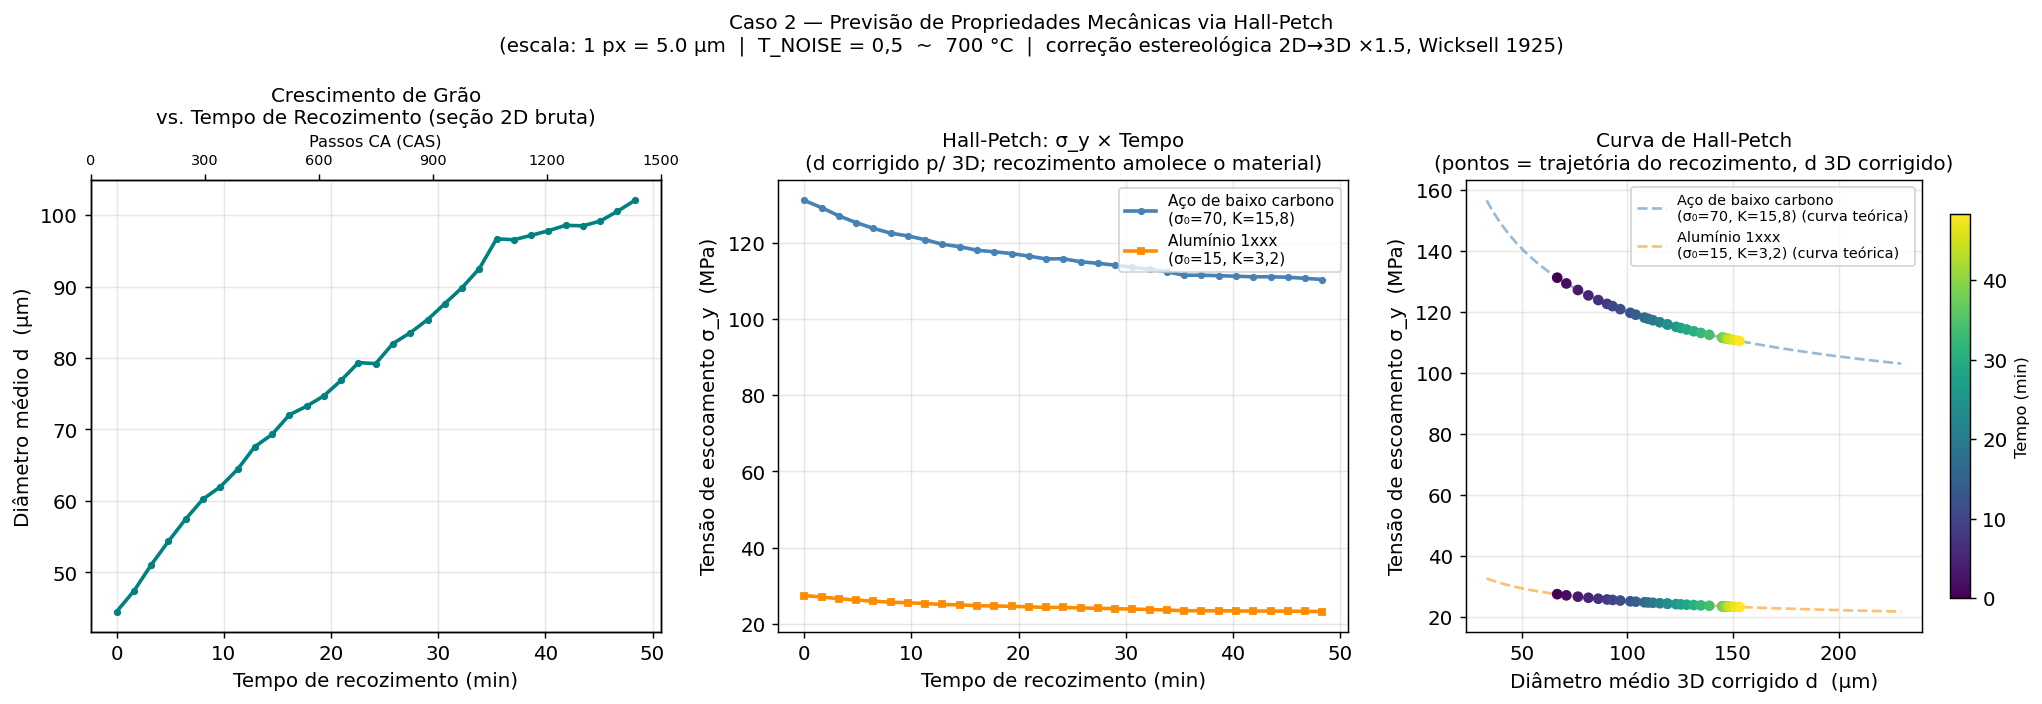
\includegraphics[width=\textwidth]{aplicacoes/resultados/caso2_hall_petch.png}
    \caption{Caso 2 — Previsão de propriedades mecânicas via Hall-Petch.
    \textit{Esquerda}: crescimento do diâmetro médio de grão (seção 2D bruta) durante
    o recozimento simulado. \textit{Centro}: tensão de escoamento $\sigma_y$ ao longo
    do tempo para os dois materiais, calculada sobre o diâmetro 3D corrigido
    (Wicksell, Equação~\ref{eq:wicksell}). \textit{Direita}: trajetória da simulação
    sobre a curva teórica de Hall-Petch (eixo em diâmetro 3D corrigido), colorida pelo
    tempo de recozimento.}
    \label{fig:caso2}
\end{figure}

Embora os dois materiais apresentem magnitudes de tensão muito distintas,
refletindo seus respectivos valores de $\sigma_0$ e $K_{HP}$, a redução percentual
de $\sigma_y$ é semelhante entre eles ($15{,}8\,\%$ para o aço e $15{,}4\,\%$ para o
alumínio), pois ambos partem da mesma trajetória de crescimento de grão $d(t)$
simulada pelo motor de AC; a pequena diferença percentual decorre exclusivamente da
diferente proporção entre $\sigma_0$ e o termo de Hall-Petch $K_{HP}/\sqrt{d}$ em
cada material. O resultado ilustra de forma quantitativa o compromisso fundamental
do tratamento térmico de recozimento: o mesmo ganho de ductilidade e capacidade de
deformação associado ao crescimento de grão tem como custo uma redução proporcional
da tensão de escoamento, informação diretamente utilizável no projeto de ciclos de
recozimento que busquem um balanço específico entre resistência e conformabilidade.
Ressalva-se que, por depender da aproximação esférica de Wicksell para a correção
2D→3D, os valores absolutos de $\sigma_y$ aqui obtidos devem ser interpretados como
ilustrativos da tendência física, não como previsão quantitativa definitiva para um
material real.

\newpage

% =====================================================================
\section{Conclusão}
% =====================================================================

Este trabalho implementou e validou uma simulação bidimensional de crescimento de
grãos em materiais policristalinos utilizando o modelo de Autômatos Celulares
Clássico com regra de mínima energia \cite{he2006, raghavan2007}, com uma extensão
estocástica que soluciona o problema fundamental dos contornos planos congelados.

As duas modificações-chave em relação à formulação puramente determinística são:
(i) aceitação probabilística de transições neutras ($\Delta E = 0$) e com aumento
de energia ($\Delta E > 0$), via parâmetros $P_{\text{neutral}}$ e $T$; e
(ii) desempate aleatório entre candidatos de energia equivalente, que elimina o
viés direcional a $45^\circ$ causado pela seleção determinística do índice 0.
Ambas as modificações preservam o caráter essencial do Autômato Celular: a
orientação proposta permanece sendo uma função determinística da vizinhança.

Os resultados demonstram que o modelo revisado reproduz os fenômenos físicos
essenciais do crescimento normal:
\begin{itemize}
    \item A cinética obedece à Lei de Burke com $R^2 = 0{,}977$, confirmando o
          comportamento parabólico previsto pela teoria;
    \item O expoente de crescimento $n = 0{,}28$ é coerente com a literatura para
          modelos CA com atualização síncrona \cite{raghavan2007, janssens2010},
          e reflete a taxa de crescimento mais conservadora da regra de mínima
          energia;
    \item A distribuição de tamanho de grão normalizada apresenta tendência à
          auto-similaridade, com parâmetros Weibull ($k = 2{,}04$) e log-normal
          ($\sigma = 0{,}591$) consistentes com a literatura \cite{wang2023, he2006};
    \item A morfologia dos grãos é fisicamente correta: contornos curvos, junções
          triplas com ângulos próximos a $120^\circ$ e ausência de viés direcional;
    \item O modelo validado foi aplicado com sucesso a dois problemas de engenharia
          de materiais: otimização de tratamento térmico calibrada fisicamente e
          previsão de propriedades mecânicas via relação de Hall-Petch. E podem ser estendidos a outros problemas de interesse,
          demonstrando seu potencial preditivo prático (Seção~\ref{sec:aplicacoes}).
\end{itemize}

O modelo CA clássico revisado é fiel ao paradigma de Autômatos Celulares, pois a
regra de transição (Equação~\ref{eq:regra_ca}) é uma função determinística do
estado da vizinhança local, e representa uma contribuição metodológica relevante
para a modelagem microestrutural de materiais policristalinos.

Como perspectivas para trabalhos futuros, destacam-se:
\begin{itemize}
    \item A implementação de atualização assíncrona (embaralhamento aleatório da
          ordem de atualização), que deve reduzir os cancelamentos síncronos e
          aumentar o expoente $n$ em direção ao valor teórico;
    \item A incorporação de anisotropia na energia de contorno (modelo de
          Read-Shockley \cite{read1950}), para simular crescimento anormal;
    \item A extensão para três dimensões, essencial para comparação com dados
          experimentais;
\end{itemize}

\newpage
\printbibliography

\end{document}
